\documentclass{article}

\setcounter{secnumdepth}{6} % cause \paragraph to be numbered, e.g. function like \subsubsubsection.
\setcounter{tocdepth}{6} % cause \paragraph to appear in TOC

\usepackage[margin=1in]{geometry}

\usepackage{tikz}
\usetikzlibrary{er,positioning}

\usepackage{hyperref}
\hypersetup{
	colorlinks,
	linkcolor=blue,
	citecolor=blue,
	urlcolor=blue
}
	


\usepackage{graphicx}
\graphicspath{{Document-images/}}


\title{Requirements Specification: Dungeons \& Dragons 5E Character Tools}
\author{Christopher Evans - https://github.com/cevans88}

\begin{document}

\maketitle

\section{Introduction}

This document is the Software Requirements Specification document for the Dungeons \& Dragons 5th Edition Character Tools application, written to conform with the IEEE's guidelines on SRS documents. It will serve to unambiguously define the requirements of the application so that efforts in later stages of the development cycle may be more focused and effective.


\subsection{Purpose}

By formally defining the requirements of the application this document benefits the project in a number of ways:

\begin{itemize}
	\item \textbf{Reduces the development effort:} Explicitly specifying the requirements at the outset of the project minimises the amount of redesign, recoding, and retesting. It can also expose omissions and inconsistencies earlier in the development cycle where such problems require less effort to rectify.
	\item \textbf{Provides a basis for validation:} Design and implementation compliance plans can be produced using this SRS as a reference.\\
\end{itemize}
It is divided into \textbf{X} parts:\\
The intended audience for this document includes the design, development, and testing teams who will find its contents invaluable as a basis for their work (whether that be designing interfaces or writing test suites to verify the meeting of specific requirements).


\subsection{Scope}
\label{sec:scope}
Application: Dungeons \& Dragons 5th Edition Character Tools\\

\noindent
The intent of the application is to provide desktop GUI tools for creating, viewing, and storing characters in the D\&D 5E ruleset. Users will be able to make selections from the various player classes, backgrounds, races, and equipment lists, as well as customise the statistics, equipment, and levels of characters once they have been created.

By consolidating all the choices that are found across the various books and supplements available to players into one application and providing a means of easily creating and viewing characters with those choices the application aims to streamline the process of planning or experimenting with characters.

Additional features which the application could be extended with include a combat simulation facility, the option of sharing or exporting character profiles with others, and implementing the suite as a web application.\\

\noindent
In order to provide an effective character creation suite it will be necessary for the application to:
\begin{itemize}
	\item Accurately model the systems present in D\&D 5E;
	\item Be up to date on all the available character options that exist across the D\&D 5E books;
	\item Since additional releases are inevitable the application should be able to easily integrate further options.
	\item Provide a GUI that:
	\begin{itemize}
		\item Is pleasing to the eye;
		\item Presents all the desired character information in a useful way, that is:
		\begin{itemize}
			\item Can all be viewed at once if needed;
			\item Can be contrasted with other options;
			\item Is self-explanatory either through labels or tooltips.				
			\item Makes it easy to make selections or edits.
		\end{itemize}
	\end{itemize}
\end{itemize}

\noindent
\\In order to provide a combat simulation facility the application will need to be extended to include:
\begin{itemize}
	\item Data for modelling the various creatures that can be involved in combat with player characters;
	\item Accurate modelling of the combat systems in D\&D5E;
	\item A suitable interface for setting up, running, and analysing combat encounters.
	\item Since D\&D5E combat is often represented as a grid of 5" by 5" squares it would make sense to base the interface around this model;
	\item The scope of this feature does not extend to implementing an artificial intelligence system for creatures in the combat scenario.
\end{itemize}

\noindent
Enabling the sharing or exporting of character profiles will require the application to be able to convert the totality of a character's attributes to a string, and in turn be able to import such a string and construct the same character entity.\\

\noindent
Implementing the suite as a web application would entail embedding it into a website so that users will not have to run an executable on their desktop computer to use the application.\\

\subsection{References}
% This subsection should:
% - Provide a complete list of documents referenced elsewhere in the SRS;
% - Identify each document by title, report number (if applicable), date, and publishing organisation;
% - Specify the sources from which the references can be obtained.

% This information may be provided by reference to an appendix or to another document.


{\setlength{\parindent}{0cm}This SRS shall be used in conjunction with the following documents:\\

D\&D5E Character Sheet, \hyperref[fig:appa]{Figure \ref{fig:appa}} in Appendix, Wizards of the Coast LLC, 28/08/2017.\\

D\&D5E Spellcasting Sheet, \hyperref[fig:appb]{Figure \ref{fig:appb}} in Appendix, Wizards of the Coast LLC, 28/08/2017.\\
}

\subsection{Definitions, acronyms, and abbreviations}
% This subsection should provide the definitions of all terms, acronyms, and abbreviations required to properly interpret the SRS. This information may be provided by reference to one or more appendixes in the SRS or by reference to other documents.

In order to fully disambiguate terms used in this SRS a number of key terms are defined below:

\subsubsection{Dungeons \& Dragons 5th Edition:}
The 5th edition rules system for the Dungeons \& Dragons roleplaying game made and owned by Wizards of the Coast LLC. Since the rules and mechanics vary between different editions of the game it is important to define which edition the application is intended to model. The rules and mechanics being modelled are found in the 5th Edition Player's Handbook, errata clarification documents, and the wide range of supplement material that is produced for players such as the 5th Edition Sword Coast Adventurer's Guide.

\subsubsection{D\&D5E:}
Acronym for Dungeon's \& Dragons 5th Edition. "5E" also used in isolation to abbreviate "5th Edition".


\subsubsection{Character:}
A character in the context of D\&D5E is an entity comprised of many different attributes that have been selected from a variety of options by a player including, but not limited to:
\begin{itemize}
	\item Name (e.g. Tiberius)
	\item Race (e.g. Dwarf)
	\item Class (e.g. Fighter)
	\item Background (e.g. Folk Hero)
\end{itemize}
A comprehensive picture of the elements that make up a character can be seen by examining the \hyperref[fig:appa]{D\&D5E Character Sheet} included in the Appendix.

\subsubsection{Player}
The person making a D\&D5E character, synonymous with "user" of the D\&D5E Character Tools application.

\subsubsection{Player's Handbook}
The core rulebook which defines most of the mechanics used in D\&D5E, often abbreviated to the PHB.

\subsection{Overview}
% This subsection should:
% - Describe what the rest of the SRS contains;
% - Explain how the SRS is organised.

TODO

\clearpage

\section{Overall description}
This section of the SRS will provide details of the factors influencing the requirements of the application, the intent being to provide a background/context which will make the requirements easier to understand.


\subsection{Product perspective}
The application is a stand-alone and does not relate to any other applications or systems. That said, constraints that must be factored into the requirements of the system are detailed below: 

\subsubsection{User interfaces}
All user interaction with the application will be done via a GUI using mouse and keyboard. User input will consist of:

\begin{enumerate}
	\item \label{item:mouseclick} Clicking navigation and selection buttons with the mouse;
	\item Brief bursts of keyboard input to enter numeric values or text fields (such as character names)
	\item Pressing keyboard shortcuts to accomplish the same as \ref{item:mouseclick}.\\
\end{enumerate}

\noindent
\emph{Screen format:}
\begin{enumerate}
	\item The application will need to provide a window that is capable of being rendered in full-screen or windowed mode, as well as able to be resized and/or minimised.
	\item A minimum screen resolution of 1024x768 will be catered for, along with a maximum of 1920x1080.
	\item A variety of aspect ratios shall be catered for:
		\begin{itemize}
			\item 4:3
			\item 16:10
			\item 16:9\\
		\end{itemize}
\end{enumerate}


\noindent
\emph{Window layouts and content}\\
All of the window layouts will be consistent with respect:
\begin{itemize}
	\item Presence and placement of generic navigation buttons (e.g. "Previous", "Quit", "Log out").
	\item Retaining the default window controls provided by the operating system whenever the application is not being rendered in full-screen mode.
\end{itemize}

\noindent
All of the window contents will be consistent with respect:
\begin{itemize}
	\item The Tab key on the keyboard shall be usable to jump between fields.
	\item Pressing F1 on the keyboard will produce a help message pop-up relating to the currently active window.
	\item Pressing F2 on the keyboard or hovering the mouse over a label should provide an explanatory tooltip.
\end{itemize}
Regarding characteristics particular to specific interfaces:
\begin{enumerate}
	\item \hypertarget{profileselection}{\textbf{Profile selection screen:}} Window where the user shall be able to create or select a profile.
		\begin{itemize}
			\item A Default profile will be available from the outset.
			\item Profiles shall be selectable via a drop-down selection box.
		\end{itemize}
	\item \hypertarget{mainmenu}{\textbf{Main menu:}} Provides menu of buttons which are used to access the various tools of the application (e.g. "Create character", "Load character").
	\item \hypertarget{creationprompt}{\textbf{Character creation mode prompt:}} Prompts user to specify how a newly created character's ability scores are generated, in line with the options available within the PHB:
		\begin{itemize}
			\item \textit{Randomly}: Where 4 6-sided dice are rolled, the lowest one is discarded, and the remainder are added together. This is done 6 times to provide an array of 6 scores ranging 3-18 (e.g. [11, 12, 9, 15, 16, 8]). The player then chooses which ability is assigned each score. The score rolling process should be transparent and depict the scores being rolled one-by-one in order to involve the player in the score rolling process.
			\item \textit{Standard array}: Instead of randomly generating values a standard array is provided to assign values from ([15, 14, 13, 12, 10, 8]). 
			\item \textit{Customised ability scores}: 27 points are granted to spend on ability scores (see Table \ref{table:customscores}):
				\begin{table}[b]
				\begin{center}
					\begin{tabular}{ ||c|c||c|c|| }
						\hline
						Score & Cost & Score & Cost\\
						\hline\hline
						8 & 0 & 12 & 4\\
						9 & 1 & 13 & 5\\
						10 & 2 & 14 & 7\\
						11 & 3 & 15 & 9\\
						\hline
					\end{tabular}
					\caption{Ability score points cost}
					\label{table:customscores}
				\end{center}
			\end{table}
		\item \textit{Manual entry}: The player has free reign to enter values from 3-18 (to account for having physically rolled a set of values or simply accommodating a player's desire to experiment).
		\end{itemize}
	\item \hypertarget{charsheet}{\textbf{Character sheet:}} Provides a character sheet displaying the chosen character's values (or a blank sheet if a new character is being created). Information will need to be laid out and formatted such that it is dense enough to minimise scrolling or tabbing between pages while maintaining readability.
		\begin{itemize}
			\item Dividing character information into separate tabs or pages containing attributes with a common thread may be recommended (e.g. 3 tabs named "Attributes and Skills", "Attacks \& Equipment", and "Proficiencies \& Traits").
			\item A ``Load character'' button should produce a pop-up window providing the option of selecting a stored character to load, entering a character import string, or specifying the location of a character file.
			\item An ``Export character'' button should produce a pop-up window containing a string representing the totality of that character's attributes as well as a button enabling storage of the character within a file.
		\end{itemize}
	\item \hypertarget{comparisontool}{\textbf{Comparison tool:}} A vertically split page with a selection box at the top of each half where a character can be selected to be displayed. In order to fit both characters' information on screen a view mode selection control will be provided (so the user can decide whether to contrast attributes, skills, or other aspects).
\end{enumerate}

\noindent
The default user interface will not provide verbose explanation of labels and fields on account of the assumed presence of mouse-over tooltips and accessible help pop-ups.

\subsubsection{Software interfaces}
The presence of an Operating System capable of running the Java Virtual Machine is assumed, otherwise there are no specific software requirements associated with running the application.

\subsubsection{Memory constraints}
Since the application is intended to be operable on relatively low performance hardware the application will be constrained to operate within a 2GB memory limit. This will ensure that the application will operate effectively on a system possessing 4GB of memory (and assuming some of that will be allocated to the operating system and other background programs).


\subsection{Product functions}
% This subsection of the SRS should provide a summary of the major functions that the software will perform. For example, an SRS for an accounting program may use this part to address customer account maintenance, customer statement, and invoice preparation without mentioning the vast amount of detail that each of those functions requires.

% Sometimes the function summary that is necessary for this part can be taken directly from the section of the higher-level specification (if one exists) that allocates particular functions to the software product. Note that for the sake of clarity:
% - The functions should be organised in a way that makes the list of functions understandable to the customer or to anyone else reading the document for the first time.
% - textual or graphical models can be used to show the different functions and their relationships. Such a diagram is not intended to show a design of a product, but simply shows the logical relationships among variables.

\begin{enumerate}
	\item \textbf{Profile creation:} The user will be able to create a new profile if they would prefer to organise the characters they create using the profile system.
	\item \textbf{Profile selection:} The user will be able to select a profile from the list of existing profiles to browse the characters associated with that profile.
	\item \textbf{Profile deletion:} The user will be able to delete any existing profiles (except the "Default" profile).
	\item \textbf{Character creation:} The user will be able to create a new character which will be associated with the profile they are using (see Figure \hyperlink{fig:profilerels}{\ref{fig:profilerels}}).
	\item \textbf{Storing characters:} The user will be able to store characters that they have created or modified in a local database on their system so that the character details can be loaded in future.
	\item \textbf{Loading characters:} The user will be able to load a previously created character from a local database. Previously loaded profiles will be listed under a "Recently accessed" window.
	\item \textbf{Deleting characters:} The user will be able to delete characters associated with the current profile, deleting the local file and that character's listing in the "Recently Accessed" window.
	\item \textbf{Modifying characters:} Once a character has been created/loaded, the user will be able to make adjustments to the various values associated with the character (e.g. increase it's level, make changes to their inventory, etc).
	\item \textbf{Export characters to a String:} The application will be able to produce a string representation of the active character sheet which the user can share so that another use may import the same character settings into their application.
	\item \textbf{Comparison of characters:} The user will be able to view and contrast a pair of characters simultaneously, selecting what aspect of the characters the display mode is focused on at that given moment.
\end{enumerate}


% Insert entity-relationship diagram for application-profile-character
\begin{figure}[b]
	\centering
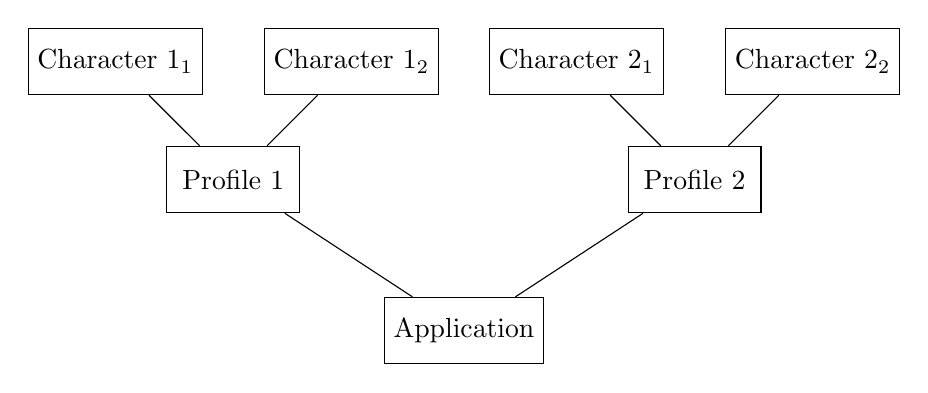
\begin{tikzpicture}[auto,node distance=1.5cm]

	\node[entity] (application) {Application};
	\node[entity] (profile1) [above left = of application] {Profile 1} 
	[grow=up, sibling distance=3cm]
	child {node[entity] {Character 1\textsubscript{2}}}
	child {node[entity] {Character 1\textsubscript{1}}} edge (application);

	\node[entity] (profile2) [above right = of application] {Profile 2} 
	[grow=up, sibling distance=3cm]
	child {node[entity] {Character 2\textsubscript{2}}}
	child {node[entity] {Character 2\textsubscript{1}}} edge (application);

\end{tikzpicture}
	\caption{Application $>$ Profile $>$ Character relationship diagram}
	\label{fig:profilerels}
\end{figure}


\subsection{User characteristics}
The intended audience of the product will be players of the D\&D5E game, as such, it is assumed that the users will be familiar with how the mechanics of the game work. Because of this the application will not be concerned with explaining how the systems work, only implementing them accurately and providing sufficient tooltip and help documentation for users to make use of the tools effectively. As an example, the application cannot assume that users will understand intuitively how to store, load, or export characters; how to make use of application features will need to be thoroughly documented.

\subsection{Apportioning of requirements}
In section \ref{sec:scope} the scope definition included descriptions of how the application could be extended to provide combat simulation tools or be converted to be run in a web browser. Both of these features are considered to be less of a priority than the other functions covered previously and consequently will not be a concern for the rest of this SRS. If a future project does start to extend the application with these features then a separate SRS will be produced. 

\clearpage
\section{Specific requirements}
% This section of the SRS should contain all of the software requirements to a level of detail sufficient to enable designers to design a system to satisfy those requirements, and testers to test that the system satisfies those requirements. Throughout this section, every stated requirement should be externally perceivable by users, operators, or other external systems. These requirements should include at a minimum a description of every input (stimulus) into the system, every output (response) from the system, and all functions performed by the system in response to an input or in support of an output. As this is often the largest and most important part of the SRS, the following principles apply:
% - Specific requirements should be stated in conformance with all the characteristics described in 4.3a.
% - Specific requirements should be cross-referenced to earlier documents that relate.
% - All requirements should be uniquely identifiable.
% - Careful attention should be given to organising the requirements to maximise readability.

% Before examining specific ways of organising the requirements it is helpful to understand the various items that comprise requirements as describe in the following sub-sections.

% Remember that the requirements in a good SRS will embody the following traits:
% - Correct;
% - Unambiguous;
% - Complete;
% - Consistent;
% - Ranked for importance and/or stability;
% - Verifiable;
% - Modifiable;
% - Traceable.


\subsection{External interface requirements}
% This should be a detailed description of all inputs into and outputs from the software system. It should complement the interface descriptions in 5.2 and should not repeat information there.

% It should include both content and format as follows:
% - Name of item;
% - Description of purpose;
% - Source of input or destination of output;
% - Valid range, accuracy, and/or tolerance;
% - Units of measure;
% - Timing;
% - Relationships to other inputs/outputs;
% - Screen formats/organisation;
% - Window formats/organisation;
% - Data formats;
% - Command formats;
% - End messages.

\subsubsection{User interfaces}

\paragraph{Startup}\mbox{}
\subparagraph{The application shall display the \protect\hyperlink{profileselection}{Profile selection screen} at program start}\mbox{} \\

\noindent
The \hyperlink{profileselection}{Profile selection screen} will be the first window to appear when the program is first executed.

\paragraph{Profile selection screen}\mbox{}
\noindent
\subparagraph{The \protect\hyperlink{profileselection}{Profile selection screen} shall display all existing profiles}
\subparagraph{The \protect\hyperlink{profileselection}{Profile selection screen} shall provide a Default profile on initial startup and thereafter}
\subparagraph{The \protect\hyperlink{profileselection}{Profile selection screen} shall provide means of creating a new profile}
\subparagraph{The \protect\hyperlink{profileselection}{Profile selection screen} shall provide means of proceeding to the \protect\hyperlink{mainmenu}{Main Menu} with a selected profile}   
\subparagraph{The \protect\hyperlink{profileselection}{Profile selection screen} shall provide means of deleting a selected profile (except the Default profile)}
\subparagraph{Pressing the F1 key on the keyboard with the \protect\hyperlink{profileselection}{Profile selection screen} active shall display a help message pop-up relating to the \protect\hyperlink{profileselection}{Profile selection screen}} 
\subparagraph{The \protect\hyperlink{profileselection}{Profile selection screen} shall include a button which can be clicked to close the application}


\paragraph{Main menu}\mbox{}
\noindent
\subparagraph{The \protect\hyperlink{mainmenu}{Main menu} shall display a collection of navigation buttons which can be clicked to access every one of the following facilities:}
\begin{enumerate}
	\item Create character;
	\item Load character;
	\item Compare character.
\end{enumerate}
\subparagraph{The \protect\hyperlink{mainmenu}{Main menu} shall include a button which can be clicked to return to the \protect\hyperlink{profileselection}{Profile selection screen}}
\subparagraph{Pressing the F1 key on the keyboard with the \protect\hyperlink{mainmenu}{Main menu} active shall display a help message pop-up relating to the \protect\hyperlink{mainmenu}{Main menu}}
\subparagraph{When the \textbf{Create character} button is clicked the user will be prompted to select how they would like to generate their character's ability scores}
\subparagraph{Pressing the \textit{1} key while the \protect\hyperlink{mainmenu}{Main menu} is active will prompt the user to select how they would like to generate their character's ability scores}
\subparagraph{When the \textbf{Load character} button is clicked the application should display the \protect\hyperlink{charsheet}{Character sheet} and immediately open a pop-up window as if the ``Load character'' button on the \protect\hyperlink{charsheet}{Character sheet} had been clicked}
\subparagraph{When the \textit{2} key is pressed the application should display the \protect\hyperlink{charsheet}{Character sheet} and immediately open a pop-up window as if the ``Load character'' button on the \protect\hyperlink{charsheet}{Character sheet} had been clicked}
\subparagraph{When the \textbf{Compare character} button is clicked the \protect\hyperlink{comparisontool}{Comparison tool} should be displayed}
\subparagraph{When the \textit{3} key is pressed the \protect\hyperlink{comparisontool}{Comparison tool} should be displayed}
\subparagraph{Pressing the \textit{Escape} key while the \protect\hyperlink{mainmenu}{Main menu} is active will return to the \protect\hyperlink{profileselection}{Profile selection screen}}


\paragraph{Character creation mode prompt}\mbox{}
\noindent
\subparagraph{The \protect\hyperlink{creationprompt}{Character creation mode prompt} shall include a button which can be clicked to return to the \protect\hyperlink{mainmenu}{Main Menu}}
\subparagraph{The \protect\hyperlink{creationprompt}{Character creation mode prompt} shall provide selection buttons and explanations of the 4 options:}
\begin{enumerate}
	\item Randomly;
	\item Standard array;
	\item Customised ability scores;
	\item Manual entry.
\end{enumerate}
\subparagraph{If the ``Randomly'' option is selected then}



\subsection{Classes/Objects}
\subsubsection{CLASS/OBJECT-ONE}
\paragraph{Attributes (direct or inherited)}
\subparagraph{ATTRIBUTE-ONE}

\paragraph{Functions (services, methods, direct or inherited)}
\subparagraph{FUNCTIONAL REQUIREMENT ONE}
% Functional requirements should define the fundamental actions that must take place in the software in accepting and processing the inputs and in processing and generating the outputs. These are generally listed as "shall" statements starting with "The system shall..."

% These include:
% - Validity checks on the inputs;
% - Exact sequence of operations;
% - Responses to abnormal situations, including:
	% - Overflow;
	% - Communication and facilities;
	% - Error handling and recovery.
% - Effect of parameters;
% - Relationship of outputs to inputs, including:
	% - Input/output sequences;
	% - Formulas for input to output conversions.

% It may be appropriate to partition the functional requirements into subfunctions or subprocesses. This does not imply that the software design will also be partitioned this way.


\paragraph{Messages (communications received or sent)}


\subsection{Performance requirements}
% This subsection should specify both the static and the dynamic numerical requirements placed on the software or on human interaction with the software as a whole. Static numerical requirements may include the following:
% - The number of terminals to be supported;
% - The number of simultaneous users to be supported;
% - Amount and type of information to be handled.

% Static numerical requirements are sometimes identified under a separate section entitled Capacity.

% Dynamic numerical requirements may include, for example, the numbers of transactions and tasks and the amount of data to be processed within certain time periods for both normal and peak workload conditions.

% All of these requirements should be stated in measurable terms.

% For example:
	% '95% of the transactions shall be processed in less than 1 s.'
% Rather than:
	% 'An operator shall not have to wait for the transaction to complete.'

% NOTE - Numerical limits applied to one specific function are normally specified as part of the processing subparagraph.



\subsection{Design constraints}
% This should specify design constraints that can be imposed by other standards, hardware limitations, etc.


\subsection{Software system attributes}
% There are a number of attributes of software that can serve as requirements. It is important that required attributes be specified so that their achievement can be objectively verified. A partial list of examples is provided below.

\subsubsection{Reliability}
% This should specify the factors required to establish the required reliability of the software system at time of delivery.

\subsubsection{Availability}
% This should specify the factors required to guarantee a defined availability level for the entire system such as checkpoint, recovery, and restart.

\subsubsection{Security}
% This should specify the factors that protect the software from accidental or malicious access, use, modification, destruction, or disclosure. Specific requirements in this area could include the need to:
% - Utilise certain cryptographical techniques;
% - Keep specific log or history data sets;
% - Assign certain functions to different modules;
% - Restrict communications between some areas of the program;
% - Check data integrity for critical variables.

\subsubsection{Maintainability}
% This should specify attributes of software that relate to the ease of maintenance of the software itself. There may be some requirement for certain modularity, interfaces, complexity, etc. Requirements should not be placed here just because they are thought to be good design practices.


\subsubsection{Portability}
% This should specify attributes of software that relate to the ease of porting the software to other host machines and/or operating systems. This may include the following:
% - Percentage of components with host-dependent code;
% - Percentage of code that is host dependent;
% - Use of a proven portable language;
% - Use of a particular compiler or language subset;
% - Use of a particular operating system.


\section{Supporting information}
% The supporting information makes the SRS easier to use. It includes the following:
% - Table of contents
% - Index
% - Appendixes

\subsection{Table of contents and index}
% The table of contents and index are quite important and should follow general compositional practices.

\subsection{Appendixes}
% The appendixes are not always considered part of the actual SRS and are not always necessary. They may include:
% - Sample input/output formats, description of cost analysis studies, or results of user surveys;
% - Supporting or background information that can help the readers of the SRS;
% - A description of the problems to be solved by the software;
% - Special packaging instructions for the code and the media to meet security, export, initial loading, or other requirements.

% When appendixes are included, the SRS should explicitly state whether or not the appendixes are to be considered part of the requirements.

\appendix

\section{D\&D5E Character Sheet}
\begin{figure}
	\centering
	\caption{D\&D5E Character Sheet}
	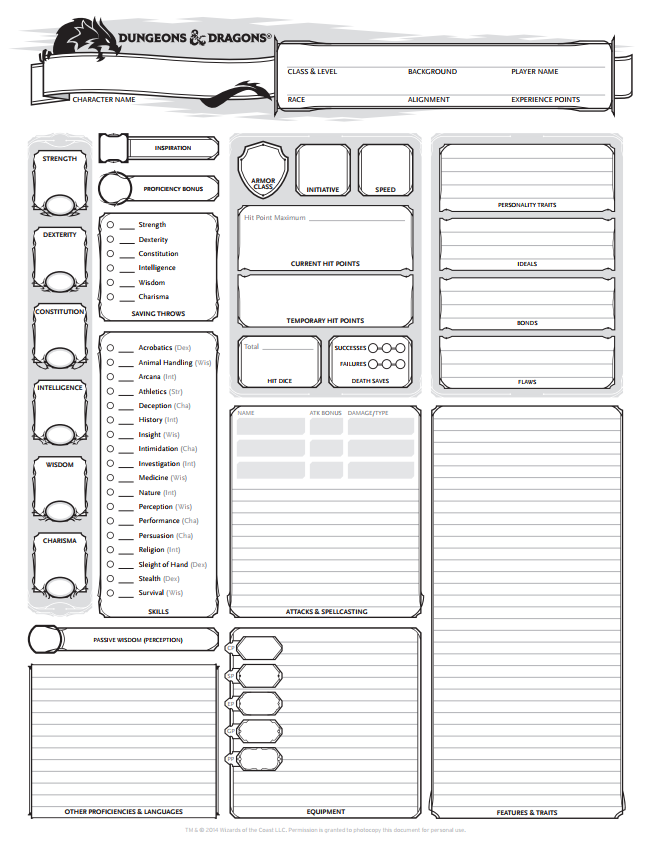
\includegraphics{character-sheet.png}
	\label{fig:appa}
\end{figure}

\section{D\&D5E Spellcasting Sheet}
\begin{figure}
	\centering
	\caption{D\&D5E Spellcasting Sheet}
	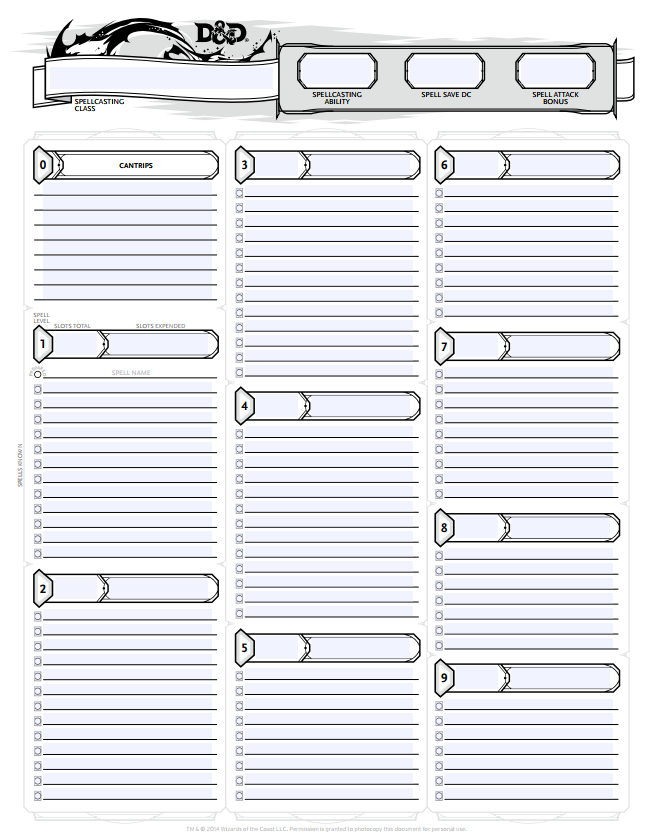
\includegraphics{spell-sheet}
	\label{fig:appb}
\end{figure}

\end{document}
